\documentclass[a4paper,11pt,english]{article}
\usepackage{geometry}
\usepackage{hyperref}
\usepackage{listings}
\usepackage{xcolor}
\usepackage{graphicx}
\usepackage{float}
\usepackage[english]{babel}

\geometry{margin=1.35in}

%%% Code style %%%

\definecolor{codegreen}{rgb}{0,0.6,0}
\definecolor{codegray}{rgb}{0.5,0.5,0.5}
\definecolor{codepurple}{rgb}{0.58,0,0.82}
\definecolor{backcolour}{rgb}{0.95,0.95,0.92}

\lstdefinestyle{mystyle}{
    backgroundcolor=\color{backcolour},   
    commentstyle=\color{codegreen},
    keywordstyle=\color{magenta},
    numberstyle=\tiny\color{codegray},
    stringstyle=\color{codepurple},
    basicstyle=\ttfamily\footnotesize,
    breakatwhitespace=false,         
    breaklines=true,                 
    captionpos=b,                    
    keepspaces=true,                 
    numbers=left,                    
    numbersep=5pt,                  
    showspaces=false,                
    showstringspaces=false,
    showtabs=false,                  
    tabsize=2
}

\lstset{style=mystyle}


\begin{document}

%%% Identification %%%

\author{
    Diogo Costa\\
    \href{mailto:up201906731@edu.fe.up.pt}{up201906731@edu.fe.up.pt}
    \and
    Francisco Colino\\
    \href{mailto:up201905405@edu.fe.up.pt}{up201905405@edu.fe.up.pt}
}
\title{FEUP -- Computer Networks \large 2021/2022 \\ \large 2.º Lab Assignment}
\date{\today}
\maketitle

%%% Summary %%%
\begin{center}
    \textbf{Summary}
\end{center}

    This report describes the steps taken to configure a computer network with 2 VLANs using 3 computers,
    1 switch, 1 Cisco router and connection to the internet to download a file with a download
    application also implemented and described in this report.
    The download application, which is a FTP client, is described first in detail. Regex was used to
    parse the URL given as argument and it uses sockets to create 2 connections (data and control connections).
    Afterwards, the network configuration and analysis is described for each of the four experiments.


%%% Introduction %%%
\section{Introduction}
    The objective of this assignment is to implement an FTP client (download application) and
    configure a computer network with 2 VLANs, composed by 3 computers, 1 switch, 1 cisco router
    and connection to the internet so that the application can be tested in it afterwards.

    In the first part of this report we describe the download application implemented and in
    the second part the network configuration.



%%% Part 1 - Download application %%%
\section{Part 1 -- Download application}
    As part of this 2nd lab assignment, we had to implement a download application that uses
    the FTP (File Transfer Protocol), described in \href{https://www.rfc-editor.org/info/rfc959}{RFC959},
    and takes an an argument that adopts the URL syntax as described in
    \href{https://www.rfc-editor.org/info/rfc1738}{RFC1738}. In this specific case, the URl is in the
    following format:
    
    $$ ftp://[<user>:<password>@]<host>/<url-path> $$
    

    %% Architecture of the download application %%
    \subsection{Architecture of the download application}
        The application has two main modules: parser and FTP client.
        The parser module takes the argument given to the application and breaks it into
        \textit{user}, \textit{password}, \textit{host}, and \textit{url-path}.
        This is accomplished using the following regular expression defined in \textit{parser.c}:

\begin{lstlisting}[language=C]
char *REGULAR_EXPRESSION = "ftp://((.+):(.+)@)?([^/@:]+)/([^\f\n\r\t\v\x20]*)";
\end{lstlisting}
        
        \noindent The function that parses the input is:
\begin{lstlisting}[language=C]
parsed_params_t* parse_input_params(const char* input);
\end{lstlisting}

        \noindent and the return structure is declared as follows in \textit{parser.h}:
\begin{lstlisting}[language=C]
typedef struct parsed_params {
    char *user;
    char *password;
    char *host;
    char *url_path;
} parsed_params_t;
\end{lstlisting}

        \noindent After the URL has been parsed into the structure, the FTP client can proceed.

        First, we need to get the IP address associated with the given \textit{host}. That is accomplished
        in the following function defined in \textit{ftp.c}:
\begin{lstlisting}[language=C]
static char *get_ip(char *host_name);
\end{lstlisting}   

        \noindent The application now creates a socket and connects it to the obtained IP in the previous step in
        the FTP control port (21). Then, it uses the \textit{user} and \textit{password} to login. The function
        that does that is defined in \textit{ftp.c}:
\begin{lstlisting}[language=C]
int ftp_login(int socket_fd, char *user, char *pass);
\end{lstlisting}

        \noindent It sends a USER command with the given \textit{user} and reads the response. If it has
        a 331 reply code (User name okay, need password.) it proceeds to send a PASS command with the
        given \textit{password} and check if the response has a 230 reply code (User logged in, proceed.)
        which indicates that the user is logged in and can now proceed to the download.

        The download is done in the following function defined in \textit{ftp.c}:
\begin{lstlisting}[language=C]
int ftp_download_file(int socket_fd, char *host, char *path);
\end{lstlisting}

        \noindent it sends a PASV command and gets the \textit{port} in the response so that it can connect
        to that port to receive the file. Then, it sends a RETR command with the given \textit{url-path} to
        the control connection and reads the file in the data connection. Once the download is finished it checks
        the reply codes to make sure the download occurred without errors.

        \noindent Finally, the application sends a QUIT command in control connection to finish the connection.


    %% Report of a successful download %%
    \subsection{Report of a successful download}
        The application was tested in several FTP servers both with username and as anonymous. The
        following image describes a usage in \textit{netlab1.fe.up.pt}:

        \begin{figure}[H]
            \centering
            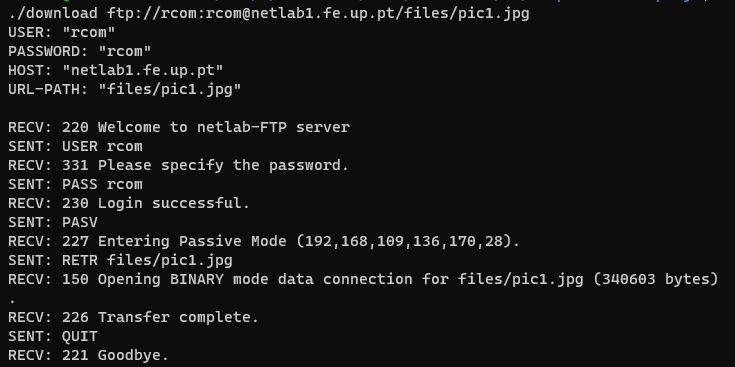
\includegraphics[scale=0.4]{./imgs/download.png}
            \caption{Successful download.}
            \label{fig:download}
        \end{figure}


%%% Part 2 - Network configuration and analysis %%%
\section{Part 2 -- Network configuration and analysis}

    %% Experiment 1 %%
    \subsection{Experiment 1}

        % Objectives %
        \subsubsection{Objectives}
            This experiment aims to configure the IP addresses of two computers and connect
            them to a Switch which should result in a network allowing both computers to
            communicate.

        % Network architecture %
        \subsubsection{Network architecture}
            This experiment uses two \textit{tux} computers (tux33, tux34) and the 
            \textit{Cisco} Switch. Each computer should be connected to the Switch 
            using an \textit{eth} port, for now both computers will use eth0. 
            
        % Main configuration commands %
        \subsubsection{Main configuration commands}
            First we need to configure the eth0 Network Interfaces on both computers, this
            is done using the following commands:

\begin{lstlisting}[language=sh]
ifconfig eth0 up                # Activates eth0 on both tuxs
ifconfig eth 0 172.16.30.1/24   # On tux33, configures it's ip address on eth0
ifconfig eth 0 172.16.30.254/24 # On tux34, configures it's ip address on eth0

route -n    # Inspect the routes that were setup
arp -a      # Check the arp tables
\end{lstlisting}
            
        % Analysis of the logs %
        \subsubsection{Analysis of the logs}
            ARP packets are used to map an IP address to a physical address (MAC). When a host wants
            to send a packet to another host, whose IP address is known but not the MAC, on the same LAN
            it first Broadcasts an ARP packet that asks for the MAC address associated with the
            destination's IP address. This is needed as Network Interface Controllers don't have IP addresses but 
            MAC addresses. We should now be able to ping the tux33 from tux34 and vice-versa.

            The ping command uses ICMP packets, these packets are sent from both origin (request) 
            and the destination (response). ICMP packets contain the Ether layer, which has both
            target and source's MAC addresses, and also contains the IP layer that holds the
            source's and target's IP addresses.

            Ethernet frames have an header, and this header has an EtherType field, this field
            is what indicates which protocol is encased in the payload (ARP, IP, ICMP, etc.), 
            the size of these frames can be determined by detecting the end of the frame that
            is usually indicated by the end of data stream symbol at the physical layer.
            A loopback interface is a virtual interface that is always active and reachable as 
            long as at least one of the switch's IP interfaces is up and running. This is important 
            due to it's address persistance, whereas interfaces or addresses of a device may change, 
            the loopback's address doesn't.


    %% Experiment 2 %%
    \subsection{Experiment 2}
        % Objectives %
        \subsubsection{Objectives}
            In this experiment, 2 virtual LANs will be setup on the switch. 
            VLAN30 composed by previously configurated tux33 and tux34, and VLAN31 composed
            by tux32. These virtual LANs will stop the tux32 from accessing tux33 and tux34,
            and vice-versa, even though they are all connected to the same switch.
            
        % Network architecture %
        \subsubsection{Network architecture}
            This experiment will use the architecture described in the experiment 1 with the
            addition of tux32 whose eth0 interface will also be connected to the switch.

        % Main configuration commands %
        \subsubsection{Main configuration commands}
            The configuration of tux33 and tux34 is the same as described in the previous
            experiment, and tux32 will be configurated in a similar fashion:

\begin{lstlisting}[language=sh]
ifconfig eth0 up                # Activates eth0
ifconfig eth0 172.16.31.1/24    # Configures it's ip address on eth0
\end{lstlisting}

            The switch also needs to be configurated which can be done by connecting one of
            the tux's serial ports to the switch controller. After accessing the Switch's
            terminal, to create the VLANs use:

\begin{lstlisting}[language=sh]
configure terminal  # Configure terminal
vlan 30             # Create VLAN 30
vlan 31             # Create VLAN 31
end                 # Exit config mode
\end{lstlisting}

            Now the ports for each VLAN have to be specified, for simplification purposes
            the ports used for each tux are:

            \begin{itemize}
                \item tux32 -- PORT 12
                \item tux33 -- PORT 3
                \item tux34 -- PORT 4
            \end{itemize}

            We now need to include ports 3 and 4 in VLAN30, and port 12 in VLAN31:

\begin{lstlisting}[caption=Adding port 3 to VLAN30]
Switch# configure terminal
Switch(config)# interface fastethernet 0/3
Switch(config-if)# switchport mode access
Switch(config-if)# switchport access vlan 30
Switch(config-if)# end
\end{lstlisting}

\begin{lstlisting}[caption=Adding port 4 to VLAN30]
Switch# configure terminal
Switch(config)# interface fastethernet 0/4
Switch(config-if)# switchport mode access
Switch(config-if)# switchport access vlan 30
Switch(config-if)# end
\end{lstlisting}

\begin{lstlisting}[caption=Adding port 12 to VLAN31]
Switch# configure terminal
Switch(config)# interface fastethernet 0/12
Switch(config-if)# switchport mode access
Switch(config-if)# switchport access vlan 31
Switch(config-if)# end
\end{lstlisting}

        % Analysis of the logs %
        \subsubsection{Analysis of the logs}
            After pinging in broadcast from tux33 and tux32 and watching where the ICMP packets
            are received we concluded that there are 2 broadcast domains, one per VLAN.


    %% Experiment 3 %%
    \subsection{Experiment 3}
        % Objectives %
        \subsubsection{Objectives}
            The objective of this experiment is to analyse the configuration of a cisco router,
            testing DNS entries and configuring routes on the local machine.

        % Network architecture %
        \subsubsection{Network architecture}
            Since this was a remote experiment, there is no network architecture.

        % Main configuration commands and analysis of the logs %
        \subsubsection{Main configuration commands and analysis of the logs}
            
            Setting static routing on is the fastest way to achieve communication in routed IP networks,
            by pointing to the next hop router which is on the way to reach destination.

\begin{lstlisting}
Router# configure terminal
Router(config)# ip route {destination} 255.255.255.0 {next hop router address}
\end{lstlisting}       
 

            \noindent NAT can be configured in a commercial Cisco router according to the \href{https://www.cisco.com/c/en/us/td/docs/ios-xml/ios/ipaddr_nat/configuration/xe-16/nat-xe-16-book/iadnat-addr-consv.html}{reference}:

\begin{lstlisting}
enable
configure terminal
ip nat inside source static local-ip global-ip
interface type number
ip address ip-address mask [secondary]
ip nat inside
exit
interface type number
ip address ip-address mask [secondary]
ip nat outside
end
\end{lstlisting}

            NAT is a method that maps multiple local IPs to a public one before transferring the information.
            This allows an organization to have multiple devices using the same public IP that can be
            accessed with different ports.

            To change the lookup table for hostnames we have to edit the /etc/hosts. For example, to add
            an entry to google with other name (youtubas) we had to add the line: 142.250.200.142 youtubas.

            DNS packets were sent before ICMP's request/reply packets, upon the use of the ping
            command, to identify the target's IP (parlamento.pt in this case).

            Concerning the Linux routing, there were ICMP packets being requested by the gateway that was routing 
            104.17.113.188 to the device to keep the connection alive. The routes setup on the device were the
            default gateway, which was removed and the route to 104.17.113.188 through 172.23.160.1 which was setup
            during the experiment.




    %% Experiment 4 %%
    \subsection{Experiment 4}
        % Objectives %
        \subsubsection{Objectives}
            First we need to add tux34 to VLAN31 and setup a route that allows
            tux33 to access tux32 through tux34. Tux32 and Tux33 should be able to access
            each other.

            The Cisco Router should be configurated in such a way that it can access 
            the Internet through the Lab Router, and added to VLAN31. This should
            allow computers that are on VLAN31 to also access the Internet.
            The final objective is to have access to the internet on tux33, since it
            can already reach devices on VLAN31 due to previous routing configuration
            all that's left is to also configure routes on the Cisco Router.

        % Network architecture %
        \subsubsection{Network architecture}
            The architecture to be used in this experiment should be close to that used
            in experiment 2 with some additions.
            Tux34 will need to have it's eth1 interface connected to the switch, using
            for example PORT 14, so that it can be added to VLAN31.
            The Cisco router GE0 interface should be connected to the Lab Router and 
            the GE1 interface to the switch, using for example PORT 19. 

        % Main configuration commands %
        \subsubsection{Main configuration commands}
            We now need to setup the tux34's IP address for interface eth1.

\begin{lstlisting}[language=sh]
ifconfig eth1 up                # Activates eth1
ifconfig eth1 172.16.31.253/24  # Configures it's ip address on eth1
\end{lstlisting}
            
            \noindent To enable port forwarding the following command must be used:
\begin{lstlisting}[language=sh]
echo 1 > /proc/sys/net/ipv4/ip\_forward
\end{lstlisting}

            \noindent The proper routes must also be setup so that tux32 and tux33 are in touch.
            On tux33:

\begin{lstlisting}[language=sh]
route add -net 172.16.31.0/24 gw 172.16.30.254 # Allows access to 172.16.31.X through tux34 (172.16.30.254)
\end{lstlisting}

            On tux32:

\begin{lstlisting}[language=sh]
route add -net 172.16.30.0/24 gw 172.16.31.253 # Allows access to 172.16.30.X through tux34 (172.16.31.253)
\end{lstlisting}

            Tux33 should now be able to communicate with every other network interface 
            (172.16.30.254, 172.16.31.253, 172.16.31.1) this can be checked by using 
            \textit{ping}.

\begin{lstlisting}[language=sh]
ping 172.16.30.254
ping 172.16.31.253
ping 172.16.31.1
\end{lstlisting}


            To configure the Cisco router its controller must be connected to one of the
            tux's serial port. After accessing the console the following command is used to
            enter config mode:

\begin{lstlisting}[language=sh]
configure terminal
\end{lstlisting}

            The configurations found in the configuration file provided
            should be adjusted and then copied to the configuration terminal:

            To configure the Interface GE0:

\begin{lstlisting}[language=sh]
interface GigabitEthernet0/0 # Interface GE0
  ip address 172.16.2.59 255.255.255.0 # IP address and mask
  ip nat outside # NAT outside as this interface should reach the Lab Router
\end{lstlisting}

            To configure the Interface GE1:
\begin{lstlisting}[language=sh]
interface GigabitEthernet0/1 # Interface GE1
  ip address 172.16.51.254 255.255.255.0 # IP address and mask
  ip nat inside # NAT inside as this interface should reach the Cisco Switch
\end{lstlisting}


            Setting up the routes to allow the Cisco Router to have access to 172.16.30.X/24:

\begin{lstlisting}[language=sh]
ip route 172.16.50.0 255.255.255.0 172.16.51.253
\end{lstlisting}

            Default gateway configuration:

\begin{lstlisting}[language=sh]
ip route 0.0.0.0 0.0.0.0 172.16.2.254
\end{lstlisting}

            The \textit{nat pool ovrld} uses IP address 172.16.2.59
            Adding the networks 172.16.30.0/24 and 172.16.31.0/24 to the access list:

\begin{lstlisting}[language=sh]
access-list 1 permit 172.16.50.0 0.0.0.7
access-list 1 permit 172.16.51.0 0.0.0.7
\end{lstlisting}

            With router's setup complete, the default gateways must be added to tux32, tux33 and tux34:

\begin{lstlisting}[language=sh]
route add default gw 172.16.31.254 # on tux32
route add default gw 172.16.30.254 # on tux33
route add default gw 172.16.31.254 # on tux34
\end{lstlisting}

        % Analysis of the logs %
        \subsubsection{Analysis of the logs}
            Tux32 has a route that allows it to access the network 172.16.30.0 via
            the IP 172.16.31.253, which belongs to Tux34, and a default gw 172.16.31.254
            to access the internet.

            Tux33 has a route that allows it to access the network 172.16.31.0 via
            the IP 172.16.30.254, which belongs to Tux34, and a default gw 172.16.30.254
            (tux34). 

            Tux34 has a default gw 172.16.31.254 to access the internet.


            \noindent Forwarding table entries contain:
            \begin{itemize} 
                \item The target's IP address/network
                \item Netmask
                \item Gateway
                \item Network Interface
                \item Metric
            \end{itemize}

            It was verified that ARP requests were sent by tux34 to determine the MAC address of 
            tux33's eth0, tux33 also sent a request to get the MAC address of tux34.
            
            The MAC addresses associated to the ICMP packets are the ones belonging to the
            origin and target devices, however due to forwarding the IP addresses associated
            might not be from the origin/target but from the device doing the forwarding.
            For example if it's between tux33 and tux32, the MAC addresses correspond to those
            two but the IP to tux34.
            


%%% Conclusions %%%
\section{Conclusions}
    This assignment allowed us to implement an FTP client (download application) and configure a computer network.
    The download application was successfully tested over the configured network.
    The analysis and discussion of the configured network allowed us to deepen our knowledge in computer networks.


%%% References %%%
\section{References}
\begin{itemize}
    \item FTP RFC -- \href{https://www.rfc-editor.org/info/rfc959}{https://www.rfc-editor.org/info/rfc959}
    \item URL RFC -- \href{https://www.rfc-editor.org/info/rfc1738}{https://www.rfc-editor.org/info/rfc1738}
    \item \href{https://www.cisco.com/c/en/us/td/docs/switches/datacenter/nexus6000/sw/unicast/7_x/cisco_n6k_layer3_ucast_cfg_rel_x/l3_route.pdf}{Configuring Static Routing}
    \item \href{https://www.cisco.com/c/en/us/td/docs/ios-xml/ios/ipaddr_nat/configuration/xe-16/nat-xe-16-book/iadnat-addr-consv.html}{Configure NAT in a commercial router}
\end{itemize}


\newpage
%%% Annexes %%%
\section{Annexes}
    %% Code of the download application %%
    \subsection{Code of the download application}

        \lstinputlisting[language=C, caption=download.c]{../src/download.c}
        
        \lstinputlisting[language=C, caption=ftp.h]{../src/ftp.h}
        
        \lstinputlisting[language=C, caption=ftp.c]{../src/ftp.c}
        
        \lstinputlisting[language=C, caption=parser.h]{../src/parser.h}
        
        \lstinputlisting[language=C, caption=parser.c]{../src/parser.c}
        
        \lstinputlisting[language=C, caption=ftp\_return\_codes.c]{../src/ftp_return_codes.h}

    %% Logs captured %%
    \subsection{Logs captured}
        \begin{figure}[H]
            \centering
            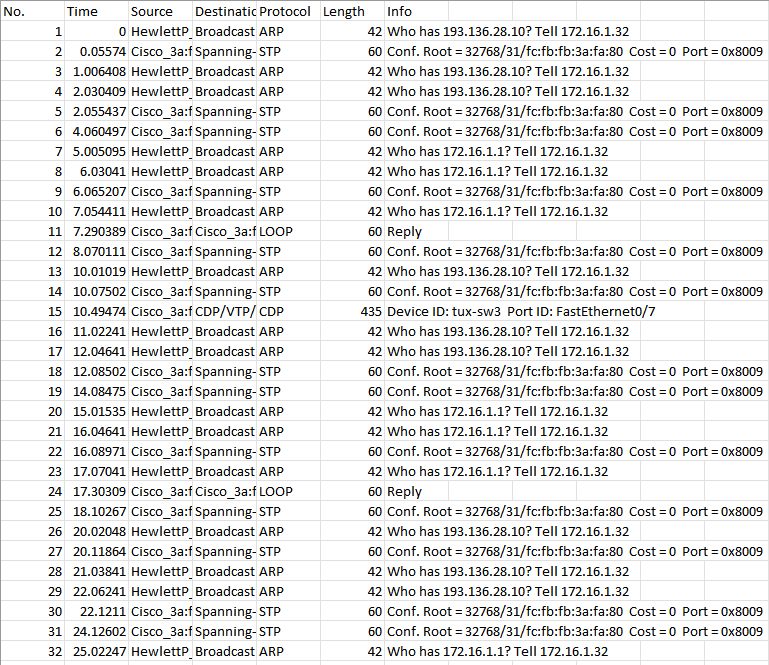
\includegraphics[scale=0.6]{./imgs/exp2-tux32-step7.png}
        \end{figure}

        \begin{figure}[H]
            \centering
            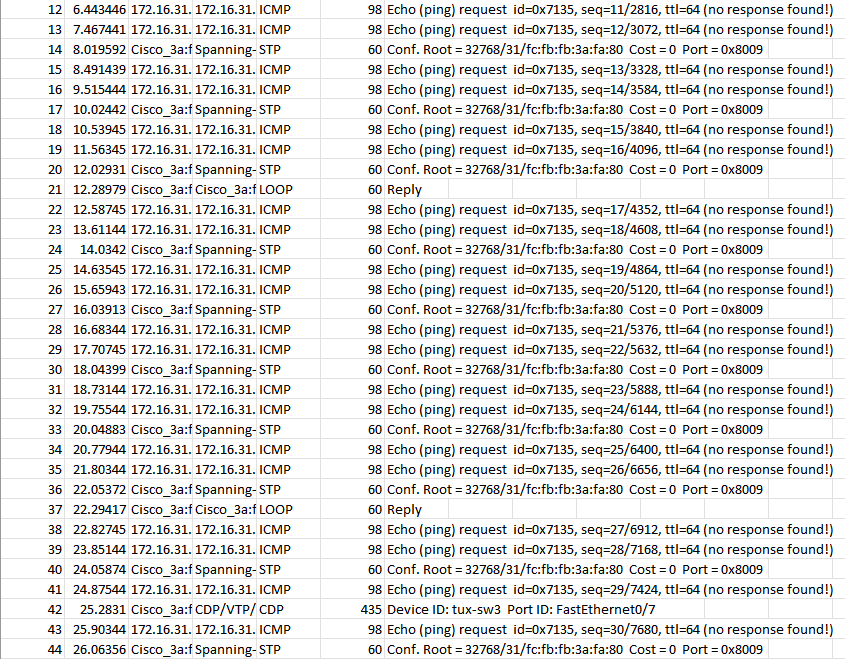
\includegraphics[scale=0.6]{./imgs/exp2-tux32-step72.png}
        \end{figure}
        
        \begin{figure}[H]
            \centering
            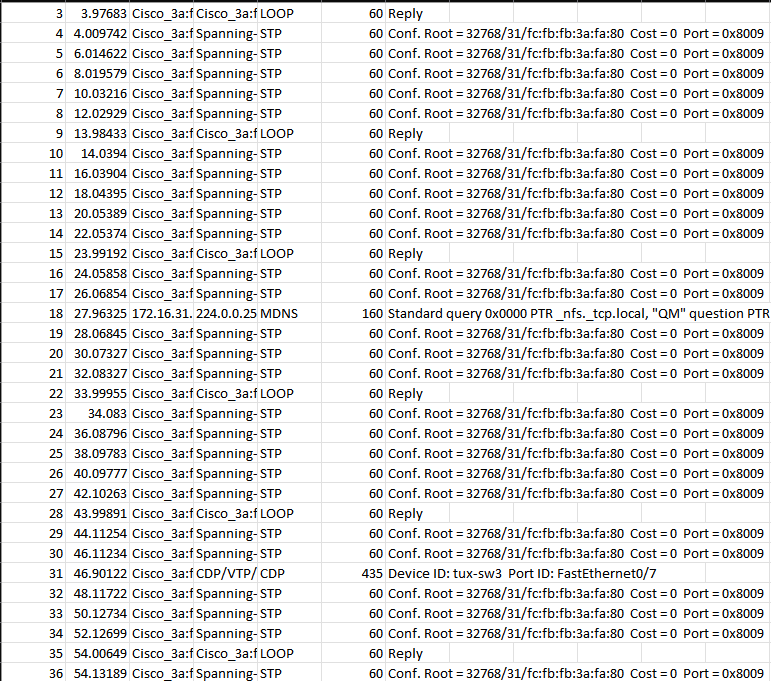
\includegraphics[scale=0.6]{./imgs/exp2-tux32-step73.png}
        \end{figure}

        \begin{figure}[H]
            \centering
            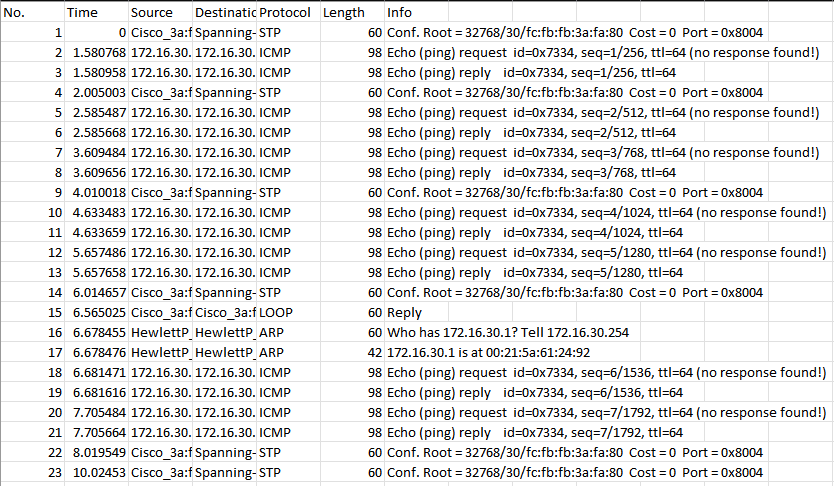
\includegraphics[scale=0.6]{./imgs/exp2-tux33-step7.png}
        \end{figure}

        \begin{figure}[H]
            \centering
            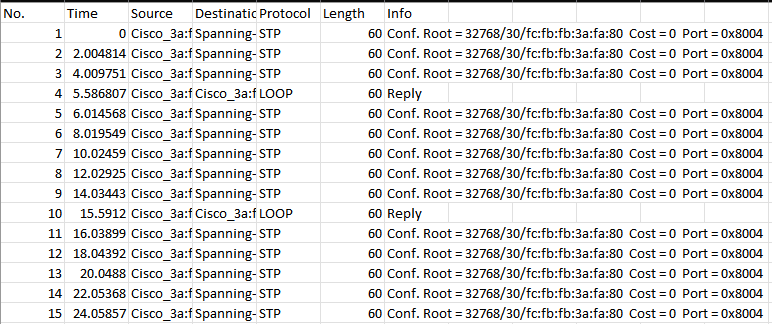
\includegraphics[scale=0.6]{./imgs/exp2-tux33-step72.png}
        \end{figure}

        \begin{figure}[H]
            \centering
            
\includegraphics[scale=0.6]{./imgs/exp2-tux33-step73.png}
        \end{figure}
        
        \begin{figure}[H]
            \centering
            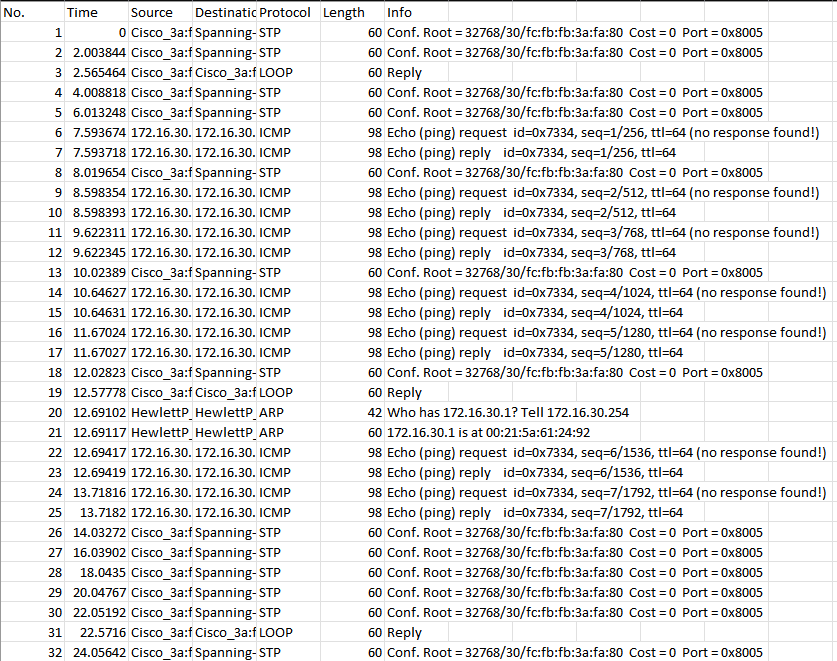
\includegraphics[scale=0.6]{./imgs/exp2-tux34-step7.png}
        \end{figure}
        
        \begin{figure}[H]
            \centering
            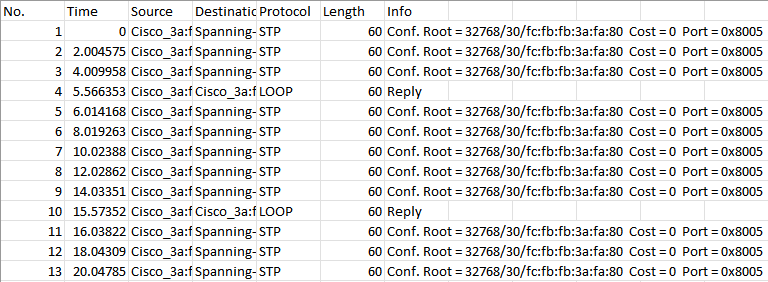
\includegraphics[scale=0.6]{./imgs/exp2-tux34-step72.png}
        \end{figure}

        \begin{figure}[H]
            \centering
            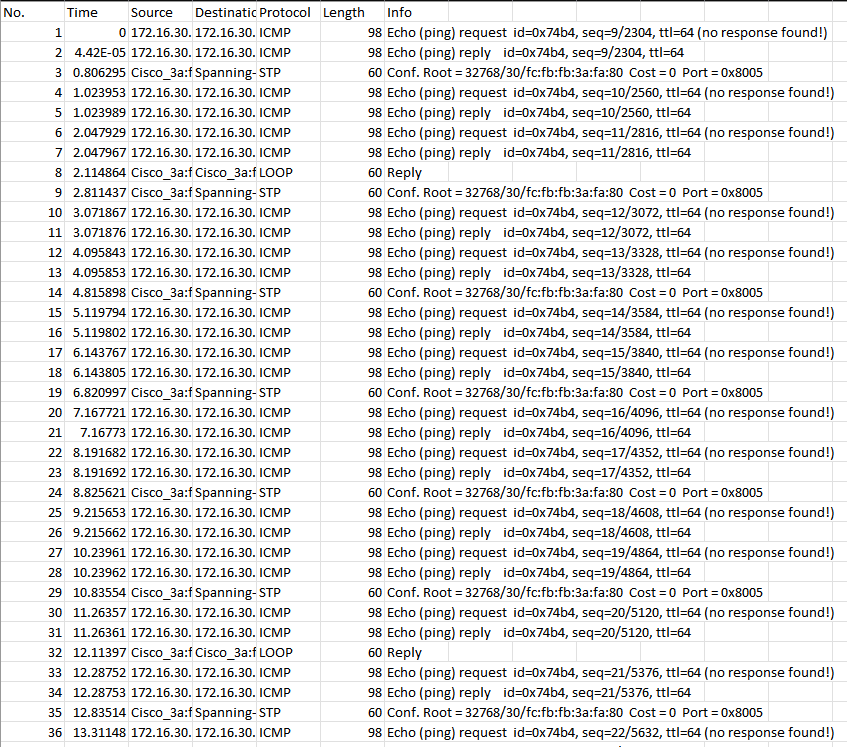
\includegraphics[scale=0.6]{./imgs/exp2-tux34-step73.png}
        \end{figure}

        \begin{figure}[H]
            \centering
            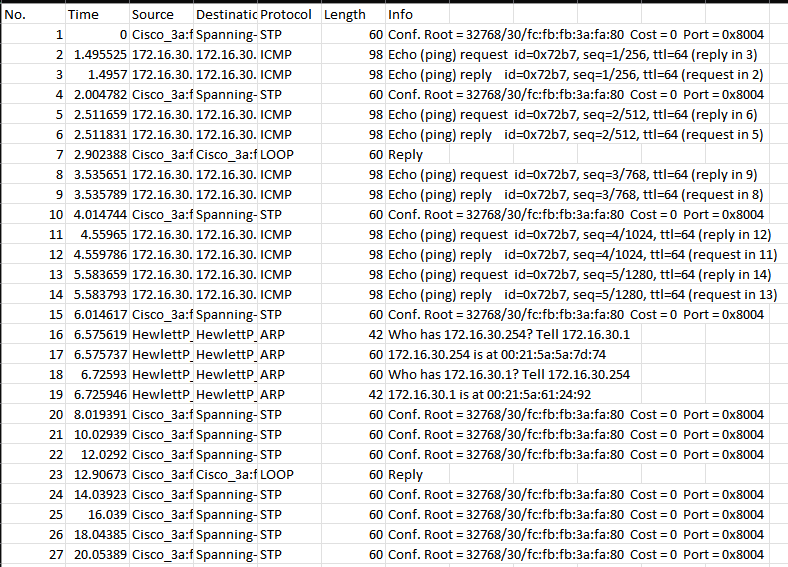
\includegraphics[scale=0.6]{./imgs/exp3-tux33-step5.png}
        \end{figure}

        \begin{figure}[H]
            \centering
            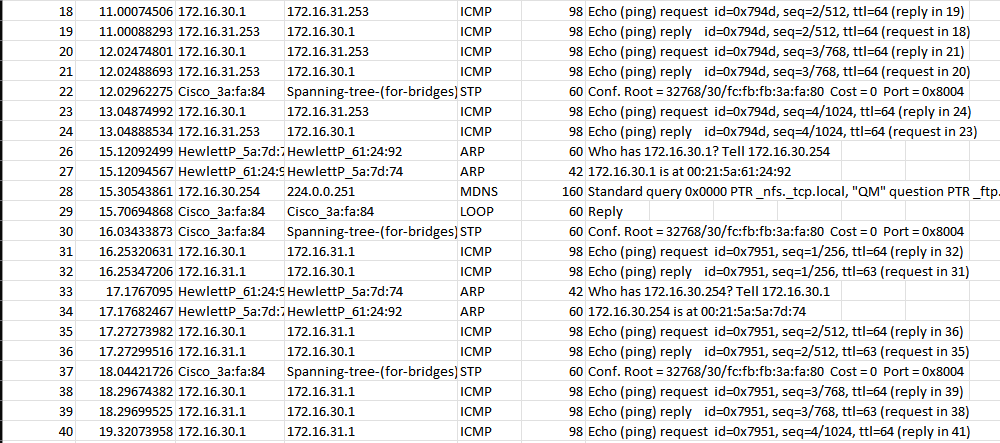
\includegraphics[scale=0.6]{./imgs/exp4-tux33-step10.png}
        \end{figure}

        \begin{figure}[H]
            \centering
            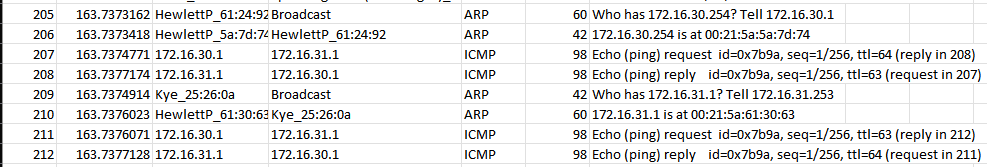
\includegraphics[scale=0.6]{./imgs/exp4-tux34-step14.png}
        \end{figure}   

\end{document}
